\subsection{Backend Implementering}

I det følgende afsnit gennemgåes implementerings detaljer omkring Web api'ets controller klasser, samt for BackEndController klassen på client siden.

\subsubsection{SaveController}

SaveController klassen består af en række HTTP metoder, disse defineres ved at anvende atributter fra librariet Mircosoft.AspNetCore.MVC, som eksempelvis HttpGet se \autoref{fig:Implementering-Backend-Code-GetSave}, der viser implementeringen af GetSave.

\begin{figure}[H]
\centering
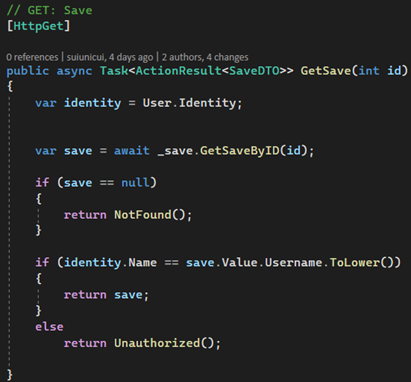
\includegraphics[width = 0.8\textwidth]{02-Body/Images/Backend_Code_GetSave.PNG}
\caption{Code snippet af HttpGet metode som modtager et id og retunere et SaveDTO object til clienten}
\label{fig:Implementering-Backend-Code-GetSave}
\end{figure}

Funkionen retunerer en Task ActionResult, som kan indeholde et SaveDTO object eller blot en status kode.

SaveController klassen tillader kun kald fra en korrekt bruger, derfor tilføjes atributten Authorize fra Microsoft.AspNetCore.Authorization librariet. User.Identity benyttes så inde i selve funktionen, til at tilgå claims for den aktuelle bruger. Herefter verificeres det, om denne brugers Username passer med det Username, som hører til det pågældende Save objekt.\\  

  
\subsubsection{UserController}

UserController klassen skal modsat SaveController klassen tillade anonyme kald, derfor tilføjes attributten AllowAnonymous. På \autoref{fig:Implementering-Backend-Code-Lgoin} ses Login funktionen.

\begin{figure}[H]
\centering
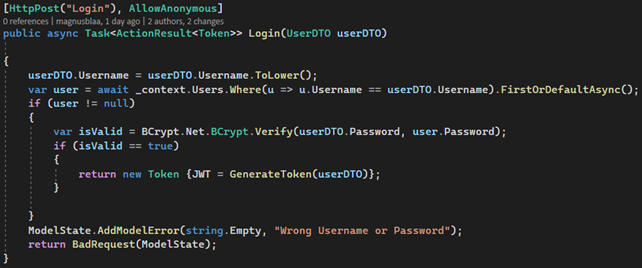
\includegraphics[width = \textwidth]{02-Body/Images/Backend_Code_Login.PNG}
\caption{Code snippet af HttpPost metode som modtager et UserDTO object og retunerer en JWT hvis brugeren findes og password’et er korrekt}
\label{fig:Implementering-Backend-Code-Lgoin}
\end{figure}

Hvis brugeren findes og pasword'et er korrekt retuneres en ny JWT, og brugeren er logget ind.\\

Til at Hashe en bruger passwords med anvendes Bcrypt \cite{Bcrypt}. Bcrypt indeholder funktionen HashPassword(”password”, BcryptWorkfactor), denne funktion skal have en BcryptWorkfactor, samt et password. Funktionen verify(”password”, hashedpassword) bruges til at verificere om et givent password svarer til dets krypterede udgave.\\


\subsubsection{BackEndController Client}

BackEndControlleren benytter sig af et HttpClient objekt til at håndtere http request/response, og et Token objekt til at holde på den modtagne JWT.
Et klasse diagram over BackEndControlleren kan ses på \autoref{fig:Implementering-Backend-Klasse-BackEndController}\\

\begin{figure}[H]
\centering
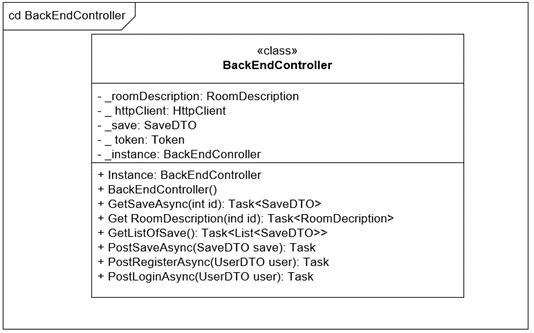
\includegraphics[width = \textwidth]{02-Body/Images/Backend_klasse_BackEndController.PNG}
\caption{klasse diagram af BackEndController}
\label{fig:Implementering-Backend-Klasse-BackEndController}
\end{figure}

BackEndController klassen implementeres som en singleton. Dette gøres for at sikre at der kun findes en JWT i programmet af gangen og for at BackEndControlleren instansen altid indeholder den korrekte JWT uanset hvorhenne i client applikationen der laves en request fra.\\


\subsubsection{Konlusion}

Backend'ens Funktioner implementeres som asynkrone funktioner, der først retunerer en værdi når resourcen som efterspørges er klar. Client klassen BackEndController implementeres som en singleton for at holde styr på den aktuelle JWT.

\newpage
